\chapter{User Guides}


\section{Running Java programs}
\label{sec:run_java}
Many of the tools that were made as part of this project were written in Java. All of them require an installation of java 7 or higher in order to run. The tools themselves are packaged inside ``JAR'' files. 

On windows, java installers automatically associate themselves with the .jar filetype. So running should only involve opening the file by double-clicking on it. The same counts for Mac OSX.

If another program has associated itself with JAR files, or the program requires command line parameters (as stated in the guide), it might be easier to run the file from the command line. The command for this is:

\begin{verbatim} java -jar [filename].jar ["parameter 1"] ["parameter 2"] \end{verbatim}

Executed from imside the directory of the JAR file. Note that it may be needed to add the Java Runtime Environment to the system PATH variable if the installation has not done so itself.



\section{Unprojection viewer}
The STL file viewer is a java application. See \ref{sec:run_java} for instructions on how to run the program.

\begin{figure}
	\centering
	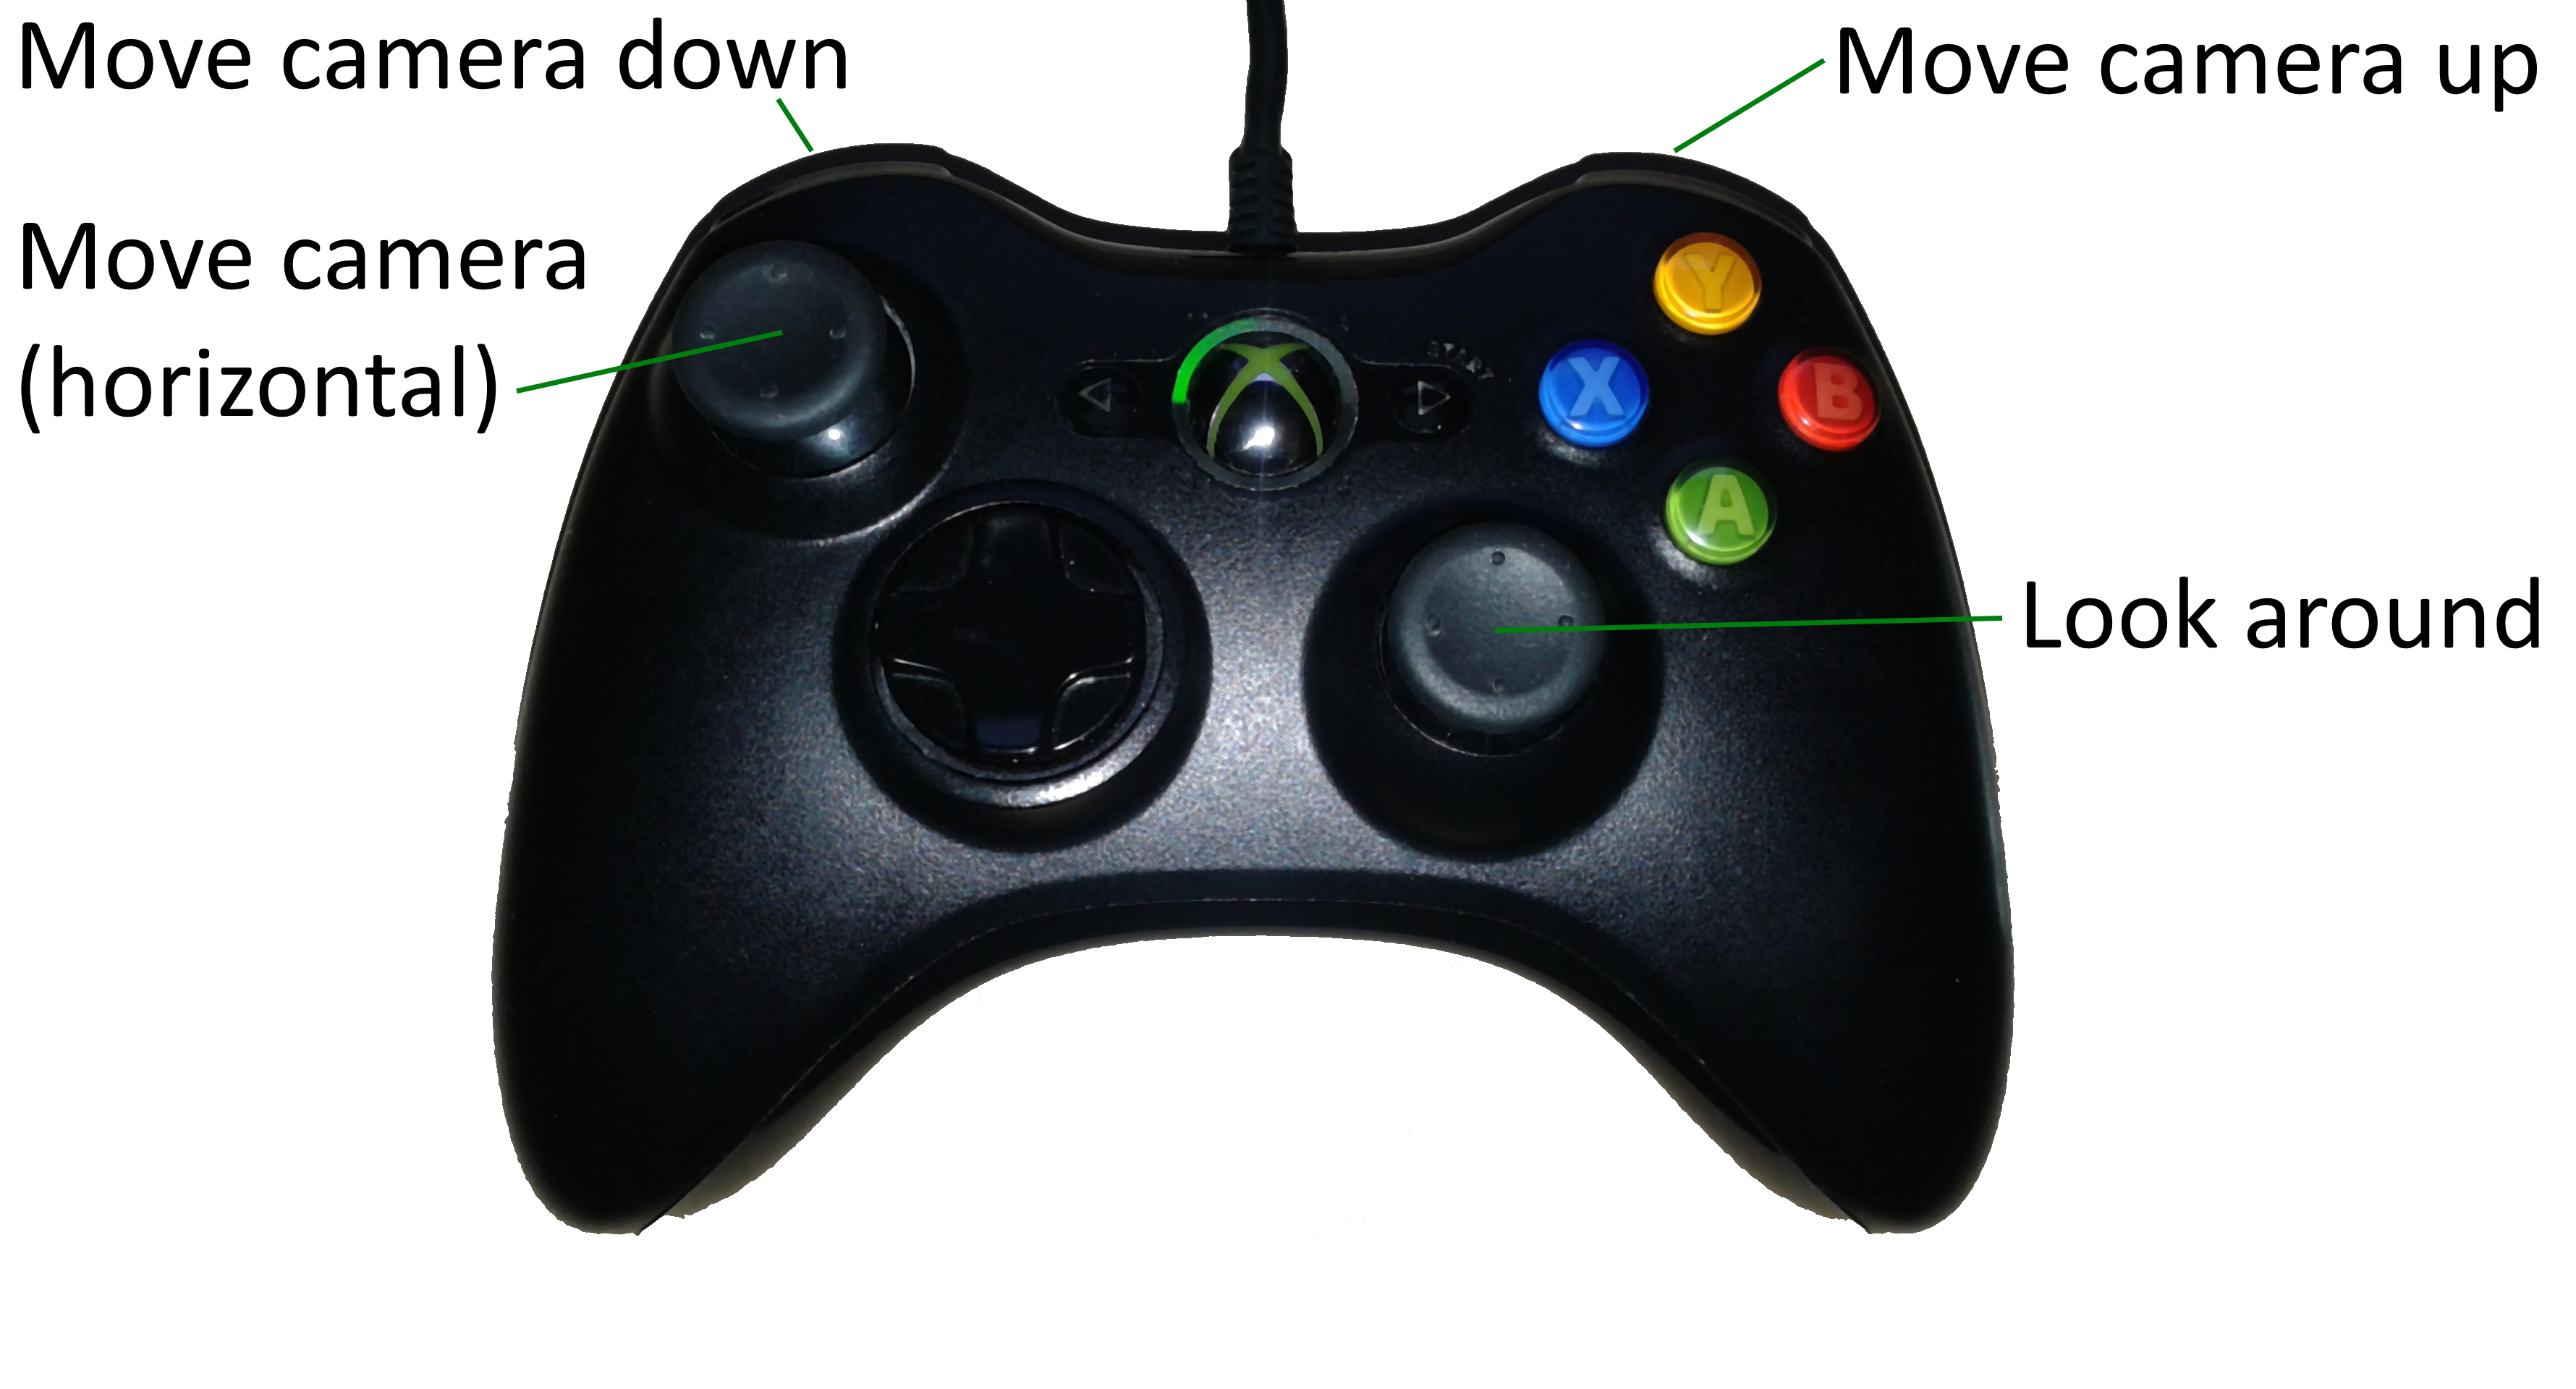
\includegraphics[width=120mm]{images/userGuide/controller_.png}
	\caption{The controls for the STL viewer and Unprojection viewer.}
	\label{fig:guide_controller}
\end{figure}

The camera of the viewer can either be controlled through an XBOX® 360 controller or a keyboard. The button layout for the controller is shown in figure \ref{fig:guide_controller}. For the keyboard controls, see table \ref{table:guide_controls}.

\begin{table}[!htb]
\centering
\begin{tabular}{|l|l|}
\hline
\textbf{Key} & \textbf{Action} \\
\hline
W & Move forward	\\
A & Move left		\\
S & Move backward	\\
D & Move right		\\
Q & Move down		\\
E & Move up			\\
Arrow keys   & Rotate camera (look around) \\
\hline
\end{tabular}
\caption{Keyboard bindings for the STL viewer and unprojection viewer}
\label{table:guide_controls}
\end{table}

\section{X-Ray simulator}

The X-Ray simulator is a java program. Section \ref{sec:run_java} explains how to run the program. The main window of the X-Ray simulator is shown in figure \ref{fig:guide_simulator}. This window is used to set up the simulation.

The window is divided vertically into two sections. The top half is used to set up the individual geometry sources and the bottom half configures amongst others the setup of the imaging. The simulator does not allow simulation of an empty scene. The button that starts the simulation is therefore initially disabled when the program is started. Geometry sources can be added by clicking the ``Add..'' button. A file selection window will pop up. Only STL files are supported by the simulator.

Once an STL file has been selected, it will appear in the geometry sources list. To remove a file from this list, select it and click the ``Remove selected'' button. The simulator requires that the density of each model is known. This can be specified for a single geometry source by selecting it in the sources list, then specifying some density in the input box to its right. Note that these boxes specify the relative density. For example, two geometry sources with relative densities will imply that the second source is twice as dense as the first, respectively.

When the geometry sources have been added and configured, the X-Ray scanning setup has to be specified. On the lower half of the screen are input boxes for the 3D coordinate of the emitter, as well as the X positions of the two detectors. 

Finally, the resolution of the image has to be specified. A recommended value is 1000 pixels. Note that larger resolutions will quickly lead to large memory usage. Also note that the image height is calculated automatically from the size of the geometry. The geometry is also scaled so that it always completely fills the image.

The fish rotation is optional, but can be used to rotate the fish around the Z-axis.

\begin{figure}
	\centering
	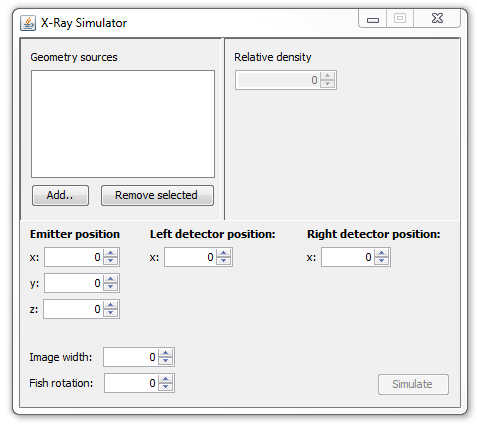
\includegraphics[width=120mm]{images/userGuide/simulator.png}
	\caption{The main window of the X-Ray simulator.}
	\label{fig:guide_simulator}
\end{figure}

\section{Bone processor}
The bone unprojector is the only program that is not a java program. Note that it has only been tested on, and compiled for windows.

Both rely on a configuration file for a number of settings. This file is located in the same directory as the executables, called ``config.cfg''. The settings in this file are:

\begin{description}
	\item[emitter.x, emitter.y, emitter.z]
		Emitter position 
	\item [fish-origin.x, fish-origin.y, fish-origin.z]
		Origin of the fish relative to the origin of the scene 
	\item [detector1.x] 
		X coordinate of detector 1
	\item [detector2.x] 
		X coordinate of detector 2
	\item [image.width, image.height] 
		The width and height of the input image(s) \\ (used for generating the output images)

	\item [bone\_reconstruction.slope\_used\_coordinate\_count]
		Number of points used for calculating the slope of a line segment during bone reconstruction
	\item [bone\_reconstruction.max\_travel\_x, bone\_reconstruction.max\_travel\_y]
		Maximum number of pixels another line segment can be separated from a bone
	\item [bone\_reconstruction.min\_bone\_size]
		The minimum required number of pixels a bone must have. It is considered noise and removed if it does not meet this minumum. 
\end{description}

Only the settings with prefix ``bone\_reconstruction'' are required for running BoneFilter.exe. All other settings are needed when performing an unprojection.

When the desired settings have been configured, the two tools are started by the following commands:

\begin{verbatim} Bonefilter.exe "path/to/image.png" "image_name" [-verbose] \end{verbatim}

The first parameter specifies what image should be processed. The second specifies the name of the image. This name is used in the file name of step images (images that are saved after every processing step). Finally, an optional parameter can be added to make the program write those step images, as well as showing more progress information in the console window. Note that this program has no output at all when verbose is turned off. It will, however, give an indication of the time used to process the image. 

The unprojection tool is used as follows:

\begin{verbatim} Unprojector.exe "path/to/left/image.png" "path/to/right/image.png" [-verbose] \end{verbatim}

As an unprojection requires a stereoscopic pair, this tool takes in two image files as parameters. The verbose parameter is again optional, and has a similar effect as the bone processing tool.